\documentclass[11pt,a4paper]{article}
\usepackage[utf8]{inputenc}
\usepackage[vietnamese]{babel}
\usepackage{amsmath,amssymb}
\usepackage[version=4]{mhchem}
\usepackage{geometry}
\geometry{top=1.5cm,bottom=1.2cm,left=1.4cm,right=1.4cm,headheight=28pt,headsep=12pt,footskip=18pt}
\usepackage{graphicx}
\usepackage{xcolor}
\usepackage{tabularx}
\usepackage{array}
\usepackage{colortbl}
\usepackage{tikz}
\usepackage{fancyhdr}
\usepackage{enumitem}
\usepackage{multido}
\usepackage{tcolorbox}

\definecolor{hfRed}{HTML}{D32F2F}
\definecolor{hfGreen}{HTML}{8BC390}
\definecolor{mainGreen}{HTML}{2E7D32}
\definecolor{solBlue}{HTML}{1565C0}
\definecolor{tableGreen}{HTML}{E8F5E9}

\usepackage{ex_test}

\pagestyle{fancy}
\fancyhf{}
\renewcommand{\headrulewidth}{0.75pt}
\renewcommand{\headrule}{\hbox to\headwidth{\color{hfGreen}\leaders\hrule height \headrulewidth\hfill}}
\renewcommand{\footrulewidth}{0.75pt}
\renewcommand{\footrule}{\hbox to\headwidth{\color{hfGreen}\leaders\hrule height \footrulewidth\hfill}}

\fancyhead[L]{\small\itshape\color{hfRed}Tài liệu lưu hành nội bộ}
\fancyhead[R]{\small\color{hfRed}Thầy \textbf{TRẦN VĂN THẠNH} - 0777.470.803}

\fancyfoot[L]{\footnotesize\itshape\color{hfRed}CS1: 6/15 Nguyễn Hoàng, P. Kim Long, TP Huế \quad|\quad CS2: 24 Đặng Thái Thân, TP Huế}
\fancyfoot[R]{\small\textbf{\color{hfRed}Trang \thepage}}

\setlength{\parindent}{0pt}
\setlength{\parskip}{2pt}

\begin{document}

\begin{minipage}[t]{0.48\textwidth}
\textbf{SỞ GD\&ĐT TP HUẾ}\\
\textbf{TRƯỜNG THPT NGUYỄN ĐÌNH CHIỂU}\\
\textit{ĐỀ CHÍNH THỨC}\\
\textit{(Đề thi có 03 trang)}
\end{minipage}
\hfill
\begin{minipage}[t]{0.48\textwidth}
\raggedleft
\textbf{\color{hfRed}ĐỀ KIỂM TRA CUỐI HỌC KÌ I}\\
\textbf{NĂM HỌC: 2025 -- 2026}\\
\textbf{Môn: HÓA HỌC -- Khối 12}\\
\textit{Thời gian làm bài: 45 phút (không kể thời gian giao đề)}\\
\textbf{MÃ ĐỀ: 1003}
\end{minipage}

\vspace{4pt}
\noindent
\textit{Họ và tên thí sinh:} \dotfill \textit{Số báo danh:} \dotfill

\vspace{3pt}
\noindent
\textit{\footnotesize Biết: $\ce{H}=1;\ \ce{Cu}=64;\ \ce{Zn}=65;\ \ce{O}=16;\ \ce{C}=12;\ \ce{Na}=23;\ \ce{Ag}=108;\ \ce{N}=14;\ \ce{S}=32;\ \ce{Cl}=35,5;\ \ce{Br}=80$.}

\vspace{3pt}
\hrule color{hfGreen} height 0.5pt

\vspace{6pt}
\begin{center}
{\Large\textbf{\color{hfRed}BẢNG ĐÁP ÁN RÚT GỌN (DÀNH CHO GIÁO VIÊN -- MÃ ĐỀ 1003)}}
\end{center}

\vspace{2pt}
\noindent
\textbf{\color{mainGreen}1. Phần I: Trắc nghiệm nhiều phương án lựa chọn (3,0 điểm)}
\begin{center}
\renewcommand{\arraystretch}{1.2}
\begin{tabular}{|c|c|c|c|c|c|c|c|c|c|c|c|c|}
\hline
\rowcolor{tableGreen}
\textbf{Câu} & \textbf{1} & \textbf{2} & \textbf{3} & \textbf{4} & \textbf{5} & \textbf{6} & \textbf{7} & \textbf{8} & \textbf{9} & \textbf{10} & \textbf{11} & \textbf{12} \\
\hline
\textbf{Đ/A} & \textbf{\color{hfRed}C} & \textbf{\color{hfRed}A} & \textbf{\color{hfRed}C} & \textbf{\color{hfRed}B} & \textbf{\color{hfRed}C} & \textbf{\color{hfRed}B} & \textbf{\color{hfRed}A} & \textbf{\color{hfRed}C} & \textbf{\color{hfRed}A} & \textbf{\color{hfRed}C} & \textbf{\color{hfRed}B} & \textbf{\color{hfRed}B} \\
\hline
\end{tabular}
\end{center}

\vspace{2pt}
\noindent
\textbf{\color{mainGreen}2. Phần II: Trắc nghiệm Đúng / Sai (2,0 điểm)}
\begin{center}
\renewcommand{\arraystretch}{1.2}
\begin{tabular}{|c|p{7.5cm}|c|c|c|c|}
\hline
\rowcolor{tableGreen}
\textbf{Câu} & \textbf{Nội dung câu hỏi} & \textbf{Lệnh a} & \textbf{Lệnh b} & \textbf{Lệnh c} & \textbf{Lệnh d} \\
\hline
\textbf{Câu 1} & Sơ đồ chuyển hóa X ($\ce{C4H8O2}$) & \textbf{\color{gray}S} & \textbf{\color{gray}S} & \textbf{\color{hfRed}Đ} & \textbf{\color{hfRed}Đ} \\
\hline
\textbf{Câu 2} & Tính chất amino acid và amine & \textbf{\color{hfRed}Đ} & \textbf{\color{gray}S} & \textbf{\color{hfRed}Đ} & \textbf{\color{hfRed}Đ} \\
\hline
\end{tabular}
\end{center}

\vspace{2pt}
\noindent
\textbf{\color{mainGreen}3. Phần III: Trắc nghiệm Trả lời ngắn (2,0 điểm)}
\begin{center}
\renewcommand{\arraystretch}{1.2}
\begin{tabular}{|c|c|c|c|c|}
\hline
\rowcolor{tableGreen}
\textbf{Câu} & \textbf{Câu 1} & \textbf{Câu 2} & \textbf{Câu 3} & \textbf{Câu 4} \\
\hline
\textbf{Đáp án} & \textbf{\color{hfRed}46} & \textbf{\color{hfRed}6} & \textbf{\color{hfRed}2} & \textbf{\color{hfRed}4,5} \\
\hline
\end{tabular}
\end{center}

\vspace{2pt}
\noindent
\textbf{\color{mainGreen}4. Tóm tắt đáp số Phần Tự luận (3,0 điểm)}
\begin{center}
\renewcommand{\arraystretch}{1.2}
\begin{tabular}{|c|c|p{11.5cm}|}
\hline
\rowcolor{tableGreen}
\textbf{Câu} & \textbf{Điểm} & \textbf{Đáp số cốt lõi} \\
\hline
\textbf{Câu 1} & 1,0 đ & CTPT $\ce{C3H7O2N}$ ($M=89$), $M(\text{muối}) = 97\text{ g/mol}$ ($\ce{H2N-CH2-COONa}$) $\Rightarrow$ CTCT của X: $\ce{H2N-CH2-COOCH3}$ (methyl glycinate). \\
\hline
\textbf{Câu 2} & 1,0 đ & $n(\ce{CuSO4}\text{ pư}) = 0,01\text{ mol}$; $n(\ce{CuSO4}\text{ dư}) = 0,005\text{ mol} \Rightarrow n(\ce{CuSO4}\text{ bđ}) = 0,015\text{ mol} \Rightarrow C_M = \mathbf{0,15\text{ M}}$. \\
\hline
\textbf{Câu 3} & 1,0 đ & $m(\text{ethanol}) = 5\,523\text{ g} \Rightarrow n(\text{glucose tt}) = 75,041\text{ mol} \Rightarrow m = 75,041 \times 180 \approx \mathbf{13\,507,34\text{ gam}}$ ($\approx 13,51\text{ kg}$). \\
\hline
\end{tabular}
\end{center}

\vspace{4pt}
\hrule color{hfGreen} height 0.5pt

\vspace{4pt}
\noindent
{\color{mainGreen}\textbf{\Large A. PHẦN TRẮC NGHIỆM: (7 điểm)}}

\vspace{3pt}
\noindent
{\color{mainGreen}\textbf{\large PHẦN I: (3,0 điểm) Câu trắc nghiệm nhiều phương án lựa chọn.}}\\
\textit{\small Thí sinh trả lời từ câu 1 đến câu 12, mỗi câu hỏi thí sinh chỉ chọn một phương án.}
\vspace{2pt}

\begin{ex}
Công thức cấu tạo dạng mạch hở của glucose là
\choice
{$\ce{[C6H7O2(OH)3]_n}$}
{$\ce{CH2OH[CHOH]3COCH2OH}$}
{\True $\ce{CH2OH[CHOH]4CHO}$}
{$\ce{CH2OH[CHOH]4CH2OH}$}

\loigiai{
Glucose là hợp chất polyhydroxy aldehyde mạch hở có công thức cấu tạo là $\ce{CH2OH[CHOH]4CHO}$.\\
\textbf{Chọn C.}
}
\end{ex}
\begin{ex}
Ester X có công thức phân tử $\ce{C4H8O2}$. Thủy phân X trong dung dịch NaOH dư, thu được sản phẩm gồm sodium propionate và alcohol Y. Công thức của Y là
\choice
{\True $\ce{CH3OH}$}
{$\ce{C3H5(OH)3}$}
{$\ce{C3H7OH}$}
{$\ce{C2H5OH}$}

\loigiai{
Sodium propionate là $\ce{C2H5COONa}$ (3 carbon). Ester X là $\ce{C4H8O2}$ nên có CTCT là $\ce{C2H5COOCH3}$. Alcohol Y là $\ce{CH3OH}$ (methanol).\\
\textbf{Chọn A.}
}
\end{ex}
\begin{ex}
Một học sinh thực hiện ba thí nghiệm ở điều kiện chuẩn và quan sát được các hiện tượng sau:\\
(1) Copper (Cu) kim loại không phản ứng với dung dịch $\ce{Pb(NO3)2}\ 1\text{ M}$.\\
(2) Lead (Pb) kim loại tan trong dung dịch $\ce{AgNO3}\ 1\text{ M}$ và xuất hiện tinh thể Ag.\\
(3) Silver (Ag) kim loại không phản ứng với dung dịch $\ce{Cu(NO3)2}\ 1\text{ M}$.\\
Trật tự nào sau đây thể hiện đúng mức độ khử của ba kim loại?
\choice
{$\text{Cu} > \text{Pb} > \text{Ag}$}
{$\text{Cu} > \text{Ag} > \text{Pb}$}
{\True $\text{Pb} > \text{Cu} > \text{Ag}$}
{$\text{Pb} > \text{Ag} > \text{Cu}$}

\loigiai{
- Từ (1): Cu không đẩy được Pb $\Rightarrow$ tính khử $\text{Pb} > \text{Cu}$.\\
- Từ (2): Pb đẩy được Ag $\Rightarrow$ tính khử $\text{Pb} > \text{Ag}$.\\
- Từ (3): Ag không đẩy được Cu (ngược lại Cu đẩy được Ag) $\Rightarrow$ tính khử $\text{Cu} > \text{Ag}$.\\
Trật tự mức độ khử: $\text{Pb} > \text{Cu} > \text{Ag}$.\\
\textbf{Chọn C.}
}
\end{ex}
\begin{ex}
Trong điều kiện thích hợp, glucose lên men tạo thành khí $\ce{CO2}$ và chất X. Tên gọi của X là
\choice
{methyl alcohol}
{\True ethyl alcohol}
{lactic acid}
{acetic acid}

\loigiai{
$\ce{C6H12O6} \xrightarrow{\text{men rượu}} 2\ce{C2H5OH} + 2\ce{CO2}\uparrow$. Chất X là ethyl alcohol (ethanol).\\
\textbf{Chọn B.}
}
\end{ex}
\begin{ex}
Công thức cấu tạo dưới đây là của carbohydrate nào?
\begin{center}
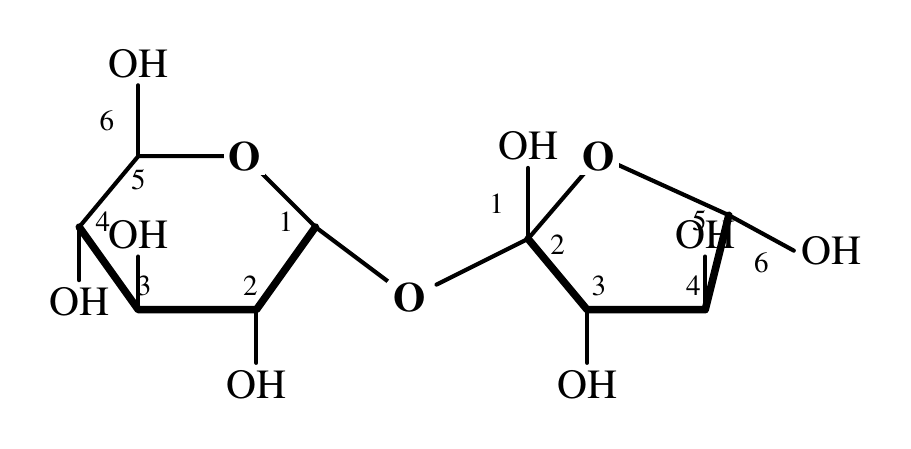
\includegraphics[width=8.0cm]{San_Pham/images_de1003/saccharose_haworth.png}
\end{center}
\choice
{glucose}
{fructose}
{\True saccharose}
{maltose}

\loigiai{
Cấu trúc gồm một gốc $\alpha$-glucose liên kết qua cầu oxy $\ce{C1-O-C2}$ với một gốc $\beta$-fructose là phân tử saccharose.\\
\textbf{Chọn C.}
}
\end{ex}
\begin{ex}
Ester có mùi đặc trưng giống mùi táo và có công thức phân tử $\ce{C5H10O2}$. Thủy phân X trong dung dịch NaOH, thu được muối sodium ethanoate và alcohol Y. Oxi hóa không hoàn toàn Y thu được chất Z có phản ứng iodoform. Công thức cấu tạo của X là
\choice
{$\ce{CH3CH2CH2COOCH3}$}
{\True $\ce{CH3COOCH(CH3)2}$}
{$\ce{CH3COOCH2CH2CH3}$}
{$\ce{CH3CH2COOCH2CH3}$}

\loigiai{
Muối sodium ethanoate là $\ce{CH3COONa}$. Ester X là $\ce{CH3COOR'}$ ($\ce{C5H10O2} \Rightarrow \ce{R'} = \ce{-C3H7}$).\\
Alcohol Y là $\ce{C3H7OH}$, bị oxi hóa tạo chất Z có phản ứng iodoform $\Rightarrow$ Y phải là propan-2-ol $\ce{CH3-CH(OH)-CH3}$, Z là acetone $\ce{CH3-CO-CH3}$.\\
Vậy X là isopropyl acetate: $\ce{CH3COOCH(CH3)2}$.\\
\textbf{Chọn B.}
}
\end{ex}
\begin{ex}
Dãy chỉ gồm các amino acid có số nhóm amino ($-\ce{NH2}$) bằng số nhóm carboxyl ($-\ce{COOH}$)?
\choice
{\True Gly, Val, Ala}
{Val, Lys, Ala}
{Gly, Ala, Lys}
{Gly, Ala, Glu}

\loigiai{
Gly, Val, Ala đều có 1 nhóm $-\ce{NH2}$ và 1 nhóm $-\ce{COOH}$. (Lys có 2 nhóm $-\ce{NH2}$; Glu có 2 nhóm $-\ce{COOH}$).\\
\textbf{Chọn A.}
}
\end{ex}
\begin{ex}
Chất nào sau đây khi đun nóng với dung dịch $\ce{H2SO4}$ loãng thu được sản phẩm có aldehyde?
\choice
{$\ce{CH3-COO-CH2-CH=CH2}$}
{$\ce{CH2=CH-COO-CH2-CH3}$}
{\True $\ce{CH3-COO-CH=CH-CH3}$}
{$\ce{CH3-COO-C(CH3)=CH2}$}

\loigiai{
$\ce{CH3COOCH=CH-CH3 + H2O <=> CH3COOH + [CH3-CH=CH-OH]}$ (enol kém bền) $\ce{-> CH3-CH2-CHO}$ (aldehyde propanal).\\
\textbf{Chọn C.}
}
\end{ex}
\begin{ex}
Từ amino acid X và methyl alcohol điều chế được ester Y có công thức phân tử $\ce{C3H7O2N}$. Công thức cấu tạo của amino acid X là
\choice
{\True $\ce{H2NCH2COOH}$}
{$\ce{CH3CH2COOH}$}
{$\ce{H2NCH2COOCH3}$}
{$\ce{CH3CH(NH2)COOH}$}

\loigiai{
Ester Y có dạng $\ce{H2N-R-COOCH3}$ ($\ce{C3H7O2N}$) $\Rightarrow \ce{R} = \ce{-CH2-}$. Amino acid X là glycine: $\ce{H2NCH2COOH}$.\\
\textbf{Chọn A.}
}
\end{ex}
\begin{ex}
Chất nào dưới đây không phải là polymer?
\choice
{Tinh bột}
{Cellulose}
{\True Lipid}
{Protein}

\loigiai{
Lipid (chất béo là triester của glycerol với acid béo) có phân tử khối khoảng vài trăm amu, không phải là hợp chất cao phân tử (polymer).\\
\textbf{Chọn C.}
}
\end{ex}
\begin{ex}
Quá trình cộng hợp liên tiếp nhiều phân tử nhỏ giống nhau hoặc tương tự nhau (monomer) tạo thành phân tử lớn (polymer) được gọi là phản ứng
\choice
{trùng ngưng}
{\True trùng hợp}
{tách}
{thế}

\loigiai{
Theo định nghĩa: Phản ứng trùng hợp là quá trình cộng hợp liên tiếp nhiều monomer tạo thành polymer.\\
\textbf{Chọn B.}
}
\end{ex}
\begin{ex}
Trong các nhận xét dưới đây, nhận xét nào đúng?
\choice
{Tất cả các chất có công thức $\ce{C_n(H2O)_m}$ đều là carbohydrate}
{\True Đa số các carbohydrate có công thức chung $\ce{C_n(H2O)_m}$}
{Phân tử các carbohydrate đều có ít nhất 6 nguyên tử carbon}
{Tất cả các carbohydrate đều có công thức chung $\ce{C_n(H2O)_m}$}

\loigiai{
Đa số các carbohydrate quen thuộc đều có công thức chung là $\ce{C_n(H2O)_m}$.\\
\textbf{Chọn B.}
}
\end{ex}
\vspace{4pt}
\noindent
{\color{mainGreen}\textbf{\large PHẦN II: (2,0 điểm) Câu trắc nghiệm đúng sai.}}\\
\textit{\small Thí sinh trả lời từ câu 1 đến câu 2. Trong mỗi ý a), b), c), d) ở mỗi câu, thí sinh chọn đúng hoặc sai.}
\vspace{2pt}

\begin{ex}
Cho sơ đồ phản ứng sau:
\begin{align*}
\ce{X}\ (\ce{C4H8O2}) + \ce{H2O} &\xrightarrow{\ce{H+}, t^\circ} \ce{Y} + \ce{Z} \\
\ce{Y} + \ce{C3H5(OH)3} &\xrightarrow{\ce{H2SO4}\ \text{đặc}, t^\circ} \ce{T} \\
\ce{Z} &\xrightarrow{\text{men giấm}} \ce{Y} \\
\ce{Z} + \ce{HCOOH} &\xrightarrow{\ce{H2SO4}\ \text{đặc}, t^\circ} \ce{W}
\end{align*}
Biết rằng X, Y, Z, T, W là các hợp chất hữu cơ khác nhau; T chỉ chứa một loại nhóm chức.
\choiceTF
{Y có trong nọc độc của kiến}
{Phần trăm khối lượng của nguyên tố oxygen trong T là $36,36\%$}
{\True Công thức cấu tạo của W là $\ce{HCOOC2H5}$}
{\True Z có trong thành phần của nước rửa tay khô có tác dụng diệt khuẩn}

\loigiai{
- $\ce{Z} \xrightarrow{\text{men giấm}} \ce{Y} \Rightarrow \ce{Z}$ là ethanol ($\ce{C2H5OH}$) và $\ce{Y}$ là acetic acid ($\ce{CH3COOH}$).\\
- $\ce{X}$ là ethyl acetate ($\ce{CH3COOC2H5}$).\\
- $\ce{T}$ là triacetin $\ce{(CH3COO)3C3H5}$ ($\ce{C9H14O6}$, $M=218\text{ g/mol}$).\\
- $\ce{W}$ là ethyl formate ($\ce{HCOOC2H5}$).\\
a) \textbf{Sai}: Y là $\ce{CH3COOH}$ (có trong giấm ăn). Acid trong nọc kiến là $\ce{HCOOH}$.\\
b) \textbf{Sai}: $\%O = (6 \times 16 / 218) \times 100\% \approx 44,04\%$ (khác $36,36\%$).\\
c) \textbf{Đúng}: $\ce{W}$ là $\ce{HCOOC2H5}$.\\
d) \textbf{Đúng}: $\ce{Z}$ là ethanol ($\ce{C2H5OH}$), cồn y tế $70-75^\circ$ dùng diệt khuẩn trong nước rửa tay khô.
}
\end{ex}
\begin{ex}
Cho các chất có công thức cấu tạo sau:
$\ce{H2NCH2COOH}$ (1); $\ce{C2H5COOH}$ (2); $\ce{C2H5NH2}$ (3); $\ce{H2NCH2CH2CH(NH2)COOH}$ (4); $\ce{C6H5NH2}$ (5).
\choiceTF
{\True Có 4 chất tác dụng được với dung dịch HCl}
{Có 1 chất tác dụng được với ethanol khi có mặt xúc tác $\ce{H2SO4}$ đặc, đun nóng}
{\True Có 3 chất tác dụng được với dung dịch NaOH}
{\True Có 2 chất vừa tác dụng được với acid vừa tác dụng được với base}

\loigiai{
a) \textbf{Đúng}: Tác dụng với $\ce{HCl}$ gồm các chất có nhóm $-\ce{NH2}$: (1), (3), (4), (5) $\Rightarrow 4$ chất.\\
b) \textbf{Sai}: Tác dụng este hóa với ethanol gồm các chất có nhóm $-\ce{COOH}$: (1), (2), (4) $\Rightarrow 3$ chất (không phải 1 chất).\\
c) \textbf{Đúng}: Tác dụng với $\ce{NaOH}$ gồm các chất có nhóm $-\ce{COOH}$: (1), (2), (4) $\Rightarrow 3$ chất.\\
d) \textbf{Đúng}: Các chất lưỡng tính vừa tác dụng với acid vừa tác dụng với base là 2 amino acid: (1) và (4).
}
\end{ex}
\vspace{4pt}
\noindent
{\color{mainGreen}\textbf{\large PHẦN III: (2,0 điểm) Câu trắc nghiệm yêu cầu trả lời ngắn.}}\\
\textit{\small Thí sinh trả lời từ câu 1 đến câu 4. Thí sinh điền kết quả vào ô trả lời tương ứng.}
\vspace{2pt}

\begin{ex}
Cao su lưu hóa có $2\%$ sulfur (S) về khối lượng. Có bao nhiêu mắt xích isoprene có một cầu disulfide ($\ce{-S-S-}$)? Giả thiết rằng S đã thay thế cho H ở cầu methylene ($-\ce{CH2}-$) trong mạch cao su.
\hfill \textbf{Trả lời:} \dotfill

\loigiai{
Một cầu disulfide ($\ce{-S-S-}$) có khối lượng $2 \times 32 = 64\text{ g/mol}$, thay thế $2\ce{H}$ ($2\text{ g/mol}$).\\
Khối lượng đoạn mạch chứa $n$ mắt xích isoprene ($\ce{C5H8}$, $M=68$): $M = 68n - 2 + 64 = 68n + 62$.\\
$\%S = \dfrac{64}{68n + 62} \times 100\% = 2\% \Rightarrow 68n + 62 = 3\,200 \Rightarrow n = \dfrac{3\,138}{68} \approx 46,15 \xrightarrow{\text{làm tròn}} \mathbf{46}$.\\
\textbf{Đáp án: 46}
}
\end{ex}
\begin{ex}
Thủy phân hoàn toàn $1\text{ mol}$ peptide mạch hở X, thu được $2\text{ mol}$ Gly, $2\text{ mol}$ Ala và $1\text{ mol}$ Val. Mặt khác, thủy phân không hoàn toàn X, thu được hỗn hợp các amino acid và các peptide (trong đó có Gly-Ala-Val). Số công thức cấu tạo phù hợp với tính chất của X là bao nhiêu?
\hfill \textbf{Trả lời:} \dotfill

\loigiai{
X là pentapeptide $(\text{Gly})_2(\text{Ala})_2(\text{Val})$.\\
Coi cụm (Gly-Ala-Val) là một khối $\text{Z}$. Hai đơn vị còn lại là 1 Gly và 1 Ala.\\
Số cấu tạo tương ứng số hoán vị 3 khối $\{\text{Gly}, \text{Ala}, \text{Z}\}$: $P_3 = 3! = \mathbf{6}$.\\
\textbf{Đáp án: 6}
}
\end{ex}
\begin{ex}
Cho các polymer sau: polybuta-1,3-diene, poly(vinyl acetate), polystyrene, nylon-6,6 và poly(phenol formaldehyde). Số polymer được điều chế bằng phản ứng trùng ngưng là bao nhiêu?
\hfill \textbf{Trả lời:} \dotfill

\loigiai{
Polymer điều chế bằng phản ứng trùng ngưng gồm: nylon-6,6 và poly(phenol formaldehyde). Tổng cộng có \textbf{2} polymer.\\
\textbf{Đáp án: 2}
}
\end{ex}
\begin{ex}
Thuỷ phân $4,4\text{ gam}$ ethyl acetate bằng $300\text{ mL}$ dung dịch NaOH $0,2\text{M}$. Sau khi phản ứng xảy ra hoàn toàn, cô cạn dung dịch, thu được $m\text{ gam}$ chất rắn khan. Giá trị của $m$ là bao nhiêu?
\hfill \textbf{Trả lời:} \dotfill

\loigiai{
$n(\text{ester}) = 4,4 / 88 = 0,05\text{ mol}$; $n(\ce{NaOH}) = 0,3 \times 0,2 = 0,06\text{ mol}$.\\
$\ce{CH3COOC2H5 + NaOH -> CH3COONa + C2H5OH}$.\\
Sau phản ứng: $n(\ce{CH3COONa}) = 0,05\text{ mol}$; $n(\ce{NaOH}\text{ dư}) = 0,06 - 0,05 = 0,01\text{ mol}$.\\
Khối lượng chất rắn khan: $m = 0,05 \times 82 + 0,01 \times 40 = 4,1 + 0,4 = \mathbf{4,5\text{ gam}}$.\\
\textbf{Đáp án: 4,5}
}
\end{ex}
\vspace{4pt}
\noindent
{\color{mainGreen}\textbf{\Large B. PHẦN TỰ LUẬN: (3 điểm)}}

\vspace{3pt}

\noindent
\textbf{Câu 1. (1,0 điểm)} Hợp chất X có công thức phân tử trùng với công thức đơn giản nhất, vừa tác dụng được với acid vừa tác dụng được với base trong điều kiện thích hợp. Trong phân tử X, thành phần phần trăm khối lượng của các nguyên tố C, H, N lần lượt bằng $40,449\%$; $7,865\%$ và $15,73\%$; còn lại là oxygen. Khi cho $4,45\text{ gam}$ X phản ứng hoàn toàn với một lượng vừa đủ dung dịch NaOH (đun nóng) thu được $4,85\text{ gam}$ muối khan. Xác định công thức cấu tạo của X.

\begin{tcolorbox}[colback=tableGreen!30,colframe=mainGreen!70,title=\textbf{Hướng dẫn giải chi tiết Câu 1},fonttitle=\bfseries]
1. Xác định công thức phân tử của X:\\
$\%O = 100\% - 40,449\% - 7,865\% - 15,73\% = 35,956\%$.\\
$n\ce{C} : n\ce{H} : n\ce{N} : n\ce{O} = \dfrac{40,449}{12} : \dfrac{7,865}{1} : \dfrac{15,73}{14} : \dfrac{35,956}{16} = 3,371 : 7,865 : 1,124 : 2,247 = 3 : 7 : 1 : 2$.\\
$\Rightarrow$ CTĐGN là $\ce{C3H7O2N} \Rightarrow$ CTPT của X là $\ce{C3H7O2N}$ ($M = 89\text{ g/mol}$).\\[4pt]
2. Xác định công thức cấu tạo của X:\\
$n(\ce{X}) = 4,45 / 89 = 0,05\text{ mol} \Rightarrow n(\text{muối}) = 0,05\text{ mol}$.\\
$M(\text{muối}) = 4,85 / 0,05 = 97\text{ g/mol}$.\\
Khối lượng mol muối tăng so với X: $97 - 89 = 8\text{ g/mol}$ chứng tỏ X là ester của amino acid:\\
$\ce{H2N-CH2-COOCH3 + NaOH -> H2N-CH2-COONa + CH3OH}$\\
Kiểm tra muối $\ce{H2N-CH2-COONa}$: $M = 16 + 14 + 44 + 23 = 97\text{ g/mol}$ (thỏa mãn).\\
$\Rightarrow$ Công thức cấu tạo của X là: $\mathbf{\ce{H2N-CH2-COOCH3}}$ (methyl glycinate).
\end{tcolorbox}

\vspace{4pt}
\noindent
\textbf{Câu 2. (1,0 điểm)} Nhúng một thanh Zn vào $100\text{ mL}$ dung dịch $\ce{CuSO4}$, sau một thời gian phản ứng lấy thanh Zn ra khỏi dung dịch, làm khô và đem cân thấy khối lượng thanh Zn giảm $0,01\text{ gam}$. Cho dung dịch loãng NaOH dư vào dung dịch sau phản ứng thu được $0,49\text{ gam}$ kết tủa. Tính nồng độ mol của dung dịch $\ce{CuSO4}$ ban đầu.

\begin{tcolorbox}[colback=tableGreen!30,colframe=mainGreen!70,title=\textbf{Hướng dẫn giải chi tiết Câu 2},fonttitle=\bfseries]
1. Phản ứng kim loại Zn đẩy Cu:\\
$\ce{Zn + CuSO4 -> ZnSO4 + Cu\downarrow}$\\
Khối lượng thanh Zn giảm: $\Delta m = m(\ce{Zn}\text{ tan}) - m(\ce{Cu}\text{ bám}) = 1\text{ mol} \times (65 - 64) = 1\text{ g/mol}$.\\
Theo đề: $\Delta m = 0,01\text{ gam} \Rightarrow n(\ce{CuSO4}\text{ pư}) = n(\ce{Zn}\text{ pư}) = \dfrac{0,01}{65 - 64} = 0,01\text{ mol}$.\\[4pt]
2. Phản ứng với dung dịch NaOH dư:\\
Dung dịch sau phản ứng chứa $\ce{ZnSO4}$ ($0,01\text{ mol}$) và $\ce{CuSO4}$ dư.\\
Khi cho NaOH loãng dư vào: kết tủa $\ce{Zn(OH)2}$ bị hòa tan hết thành $\ce{Na2[Zn(OH)4]}$.\\
Kết tủa thu được chỉ là $\ce{Cu(OH)2}$:\\
$\ce{CuSO4 (dư) + 2NaOH -> Cu(OH)2\downarrow + Na2SO4}$\\
$n[\ce{Cu(OH)2}] = 0,49 / 98 = 0,005\text{ mol} \Rightarrow n(\ce{CuSO4}\text{ dư}) = 0,005\text{ mol}$.\\[4pt]
3. Nồng độ mol dung dịch $\ce{CuSO4}$ ban đầu ($V = 0,1\text{ L}$):\\
$n(\ce{CuSO4}\text{ bđ}) = n(\text{pư}) + n(\text{dư}) = 0,01 + 0,005 = 0,015\text{ mol}$.\\
$C_M(\ce{CuSO4}) = \dfrac{0,015}{0,1} = \mathbf{0,15\text{ M}}$.
\end{tcolorbox}

\vspace{4pt}
\noindent
\textbf{Câu 3. (1,0 điểm)} Để sản xuất $10\text{ L}$ cồn y tế $70^\circ$ người ta cần lên men tối thiểu $m\text{ gam}$ glucose. Biết hiệu suất của quá trình lên men là $80\%$, khối lượng riêng của ethanol là $0,789\text{ g/mL}$. Giá trị của $m$ là bao nhiêu?

\begin{tcolorbox}[colback=tableGreen!30,colframe=mainGreen!70,title=\textbf{Hướng dẫn giải chi tiết Câu 3},fonttitle=\bfseries]
1. Khối lượng và số mol ethanol trong $10\text{ L}$ cồn $70^\circ$:\\
$V(\text{ethanol}) = 10 \times 0,70 = 7\text{ L} = 7\,000\text{ mL}$.\\
$m(\text{ethanol}) = 7\,000 \times 0,789 = 5\,523\text{ gam}$.\\
$n(\text{ethanol}) = \dfrac{5\,523}{46} \approx 120,0652\text{ mol}$.\\[4pt]
2. Tính lượng glucose tối thiểu cần dùng ($H = 80\% = 0,8$):\\
$\ce{C6H12O6 -> 2 C2H5OH + 2 CO2}$\\
$n(\text{glucose lt}) = \dfrac{n(\text{ethanol})}{2} = \dfrac{120,0652}{2} = 60,0326\text{ mol}$.\\
$n(\text{glucose tt}) = \dfrac{60,0326}{0,8} \approx 75,0408\text{ mol}$.\\
$m = 75,0408 \times 180 \approx \mathbf{13\,507,34\text{ gam}}$ ($\approx 13,51\text{ kg}$).
\end{tcolorbox}

\vspace{8pt}
\begin{center}
\textbf{---------- HẾT ----------}
\end{center}

\end{document}
